There exist many ways to realize an IMP system. Based on the previously analyzed requirements of users and OZG systems, a possible solution for an IMP system is presented.

\subsection{Components}
The IMP system operates on three domains and consists 3 system components. The user domain contains systems, a user directly interacts with. As for the system architecture of the OZG, can be a web browser. The solution for the IMP system provides an IMP client as an app for smartphones. The IMP domain contains systems hosted by the IMP provider. The IMP server is part of this domain. The Service Provider domain contains the system architecture of the service provider and integration components of the IMP solution.
In the following sections, IMP client and IMP server are explained in more detail, the integration system will be the focus of the next chapter.

\begin{figure}[h]
\caption{Overview IMP System}
    \centering
    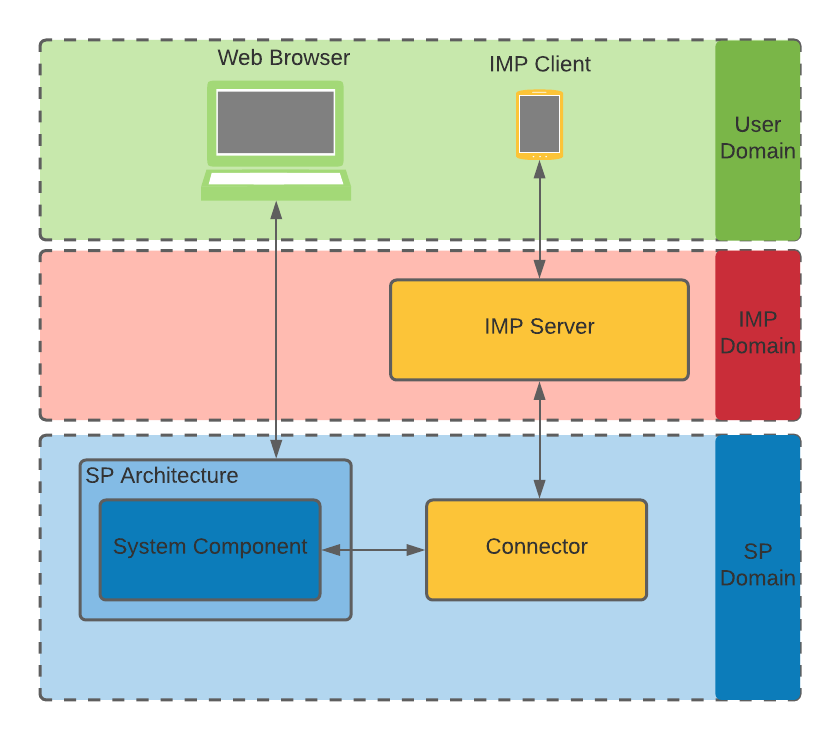
\includegraphics[scale=0.25]{Diagrams/IMP System Overview.png}
\end{figure}

\subsubsection{IMP Client}

The IMP client is a smartphone application which enables the user to manage his IMP identity. It enables the user to:

\paragraph{Create an IMP identity}

After the user installs the application on his smartphone, he is able to create an IMP identity. The identity consists of a public and private key-pair. The private key will never leave the smartphone. The public key is shared with the IMP server along with information on how to communicate with the client.

\paragraph{Manage Attributes}

The user is able to add, remove, update and read any key-value pair as an attribute of his identity. Attributes are encrypted with the 

\paragraph{Documents}

The user is able to add, remove, update and read any document as an attribute of his identity. All documents are stored on the smartphone. 

\paragraph{Send and Receive Messages}
\paragraph{Send and Receive Relationship Requests}
\paragraph{Send and Receive Share Requests}
\paragraph{Display Forms}

\subsubsection{IMP Server}
The IMP server interacts with the clients in order to deliver information from one client to the other. The server has the following functionalities:
\begin{itemize}
    \item Store identities
    \item Create and store relationship template
    \item Create and store request template
    \item Deliver relationship requests
    \item Deliver requests
    \item Deliver messages
\end{itemize}

\subsection{Functionalities}
As already introduced, the IMP solution provides the user with multiple functionalities. In this section, important features are described in more detail.

\subsubsection{Relationship}

IMP identities can establish an IMP relationship. Through this relationship, both identities can securely share attributes and communicate.

To establish a relationship, a relationship template is required. The template is created by an identity which wants to receive relationship requests and is shared with the identity which wants to request a relationship. The relationship template is stored on the IMP server and can be retrieved trough template ID. Besides technical information, the template usually contains:
\begin{enumerate}
    \item Information which the templator would like to share about itself 
    \item Information which the templator would like the requestor to share
    \item Requested additional information about the requestor 
    \item Meta information 
\end{enumerate}

\subsubsection{Share Attribute}

\subsubsection{Change Attribute}

